%!TEX root = ../../thesis.tex

\section{Exploiting overlap between distributions}
\label{chapter:limitations:overlap}


In this section, we propose a method that uses the overlap between the model for each class to identify the correct task hypothesis, and demonstrate the efficiency of our uncertainty measure on the signal space presented in chapter~\ref{chapter:planning:uncertaintysignalspace}. We present simulated experiments using pre-recorded EEG signals, and show that we achieve similar performances than calibration based systems. Finally, we report online experiments where four users control, by means of a BCI, an agent on a virtual world to reach a target without any previous calibration process.

\subsection{Using the Bhattacharyya coefficient}

Following \cite{blankertz2010single}, we model the EEG signals using independent multivariate normal distributions for each class ($\mathcal{N}(\mu_c, \Sigma_c)$ and $\mathcal{N}(\mu_w, \Sigma_w)$). We will denote by $\theta$ this set of parameters $\{\mu_c, \Sigma_c,\mu_w, \Sigma_w\}$.

We propose to exploit the fact that when labels are mixed, the Gaussian corresponding to each classes should overlap more than for the correct label association (see Figure~\ref{fig:TworldLabelGaussian}). The Bhattacharyya coefficient measures this overlap, it has been related to the classification error of Gaussian models \cite{Kailath67} and is inversely proportional to the classification rate. Although there is no analytical relation between the coefficient and the classification rate, it is possible to derive bounds and good empirical approximations \cite{lee2000bayes}.

The Bhattacharyya coefficient $\rho \in [0,1]$ between the Gaussian distributions associated to label ``correct'' ($\mathcal{N}(\mu_c, \Sigma_c)$) and ``incorrect'' ($\mathcal{N}(\mu_w, \Sigma_w)$) is:

\begin{eqnarray}
\rho = e^{-D_B(\theta)}
\end{eqnarray}

where $D_B$ is the Bhattacharyya distance:

\begin{eqnarray}
D_B(\theta) = \frac{1}{8}(\mu_c-\mu_w)^T(\frac{\Sigma_c+\Sigma_w}{2})^{-1}(\mu_c-\mu_w)+\frac{1}{2}ln\left(\frac{det(\frac{\Sigma_c+\Sigma_w}{2})}{\sqrt{det\Sigma_c det\Sigma_w}}\right)
\end{eqnarray}

Finally, we approximate the expected classification rate as:
\begin{eqnarray}
Ecr \propto 1 - \rho
\end{eqnarray}

Now that we have an estimation of the expected classification rate, which is proportional to the overlap between the model of each class, we need to take a decision with respect to which task is the one intended by the user. To do so we compare the expected classification rate of every task hypothesis $\xi_t$ with $t \in \{1, \ldots, T\}$. 

The hypothesis whose associated model overlaps the less, i.e. which has the highest expected classification rate, i.e.\ the lowest value of $\rho$, is expected to be the one intended by the user. However it is meaningless to define an absolute threshold on the value of the expected classification rate itself. Indeed, different people generate different signals which result in classifiers of different qualities. Also, even the for the correct signal-label pairs, the model may overlap by quite some amount, as shown in our 2 dimensional examples in Figure~\ref{fig:datasetsquality}. To bypass this problem we rely on a voting system where we attribute to each hypothesis $\xi_t$ a weight that is updated at every iteration.

We rely on a pseudo-likelihood metric that for each hypothesis $\xi_t$ accumulates the expected classification rate over time:

\begin{eqnarray}
\L(\xi_t) = \prod_{i = 1}^{M} 1 - \rho_i^{\xi_t}
\end{eqnarray}
%
with $M$ the current number of iteration and $\rho_i^{\xi_t}$ the Bhattacharyya coefficient associated to task $\xi_t$ using all data up to time $i$. By normalizing the pseudo-likelihood values between every hypothesis, we obtain what can be viewed as the probability of each target:

\begin{eqnarray}
p(\xi_t) = \frac{\L(\xi_t)}{\sum_{u \in \{1, \ldots, T\}} \L(\xi_u)}
\end{eqnarray}

Once a target reaches a probability threshold $\beta$ we consider it as being the correct one, i.e.\ the one intended by the user. We used $\beta = 0.99$.

Finally, once we identified the first target, we will switch back to a classification based algorithm as described in chapter~\ref{chapter:lfui:tasttotask} and as used in the previous chapters of this thesis. We will see in section~\ref{chapter:limitations:overlap:offline} that this switch is necessary to maintain good performances since the classifier makes a much harder decision for each new EEG signal.

\subsection{Planning}

As we are using a model based method, we rely on our method measure that measure uncertainty directly in the signal space. This method was described in chapter~\ref{chapter:planning:uncertaintysignalspace} and to summarize rely on computing, for every state-action pairs, the similarity between the expected signals for each task. The more the expected signals are similar the less there is uncertainty.

For computing the similarity between two Gaussian distributions we could rely again on the Bhattacharyya coefficient describe above. However computing this coefficient between all models and for all state-action pairs was not feasible in real time. In order to improve computation efficiency we do not rely on a precise metric between Gaussian distributions and only consider the similarity between their means. The closest the means are, the more similar they are.

\subsection{Offline analysis}
\label{chapter:limitations:overlap:offline}

The objective of the offline analysis is to study the impact of our exploration method and evaluate if the classifier learned from scratch with our algorithm can be reused for learning new tasks. To ensure we have sufficient data to achieve statistically significant results, we rely on a large dataset of real EEG data. We used the same dataset as describe in chapter~\ref{chapter:bci:EEGsignals} dataset from \cite{iturrate2013task}, which covers ten subjects that performed two different control problems.

For each subject, we simulated 20 runs of 400 iterations following the control task. Each time the device performed an action, we sampled the dataset using the ground truth labels corresponding to the correct task and then removed the chosen signal from it. After a first task was identified we continued running the system to identify new tasks. 

We present most of the results in terms of the quality of the dataset, measured as the classification accuracy that a calibrated brain signal classifier would obtain.

\paragraph{Planning Methods}

We compared the average number of steps (with maximum values of 400 steps) needed to identify the first task when learning from scratch with different planning methods.

\begin{figure}[!ht]
    \centering
    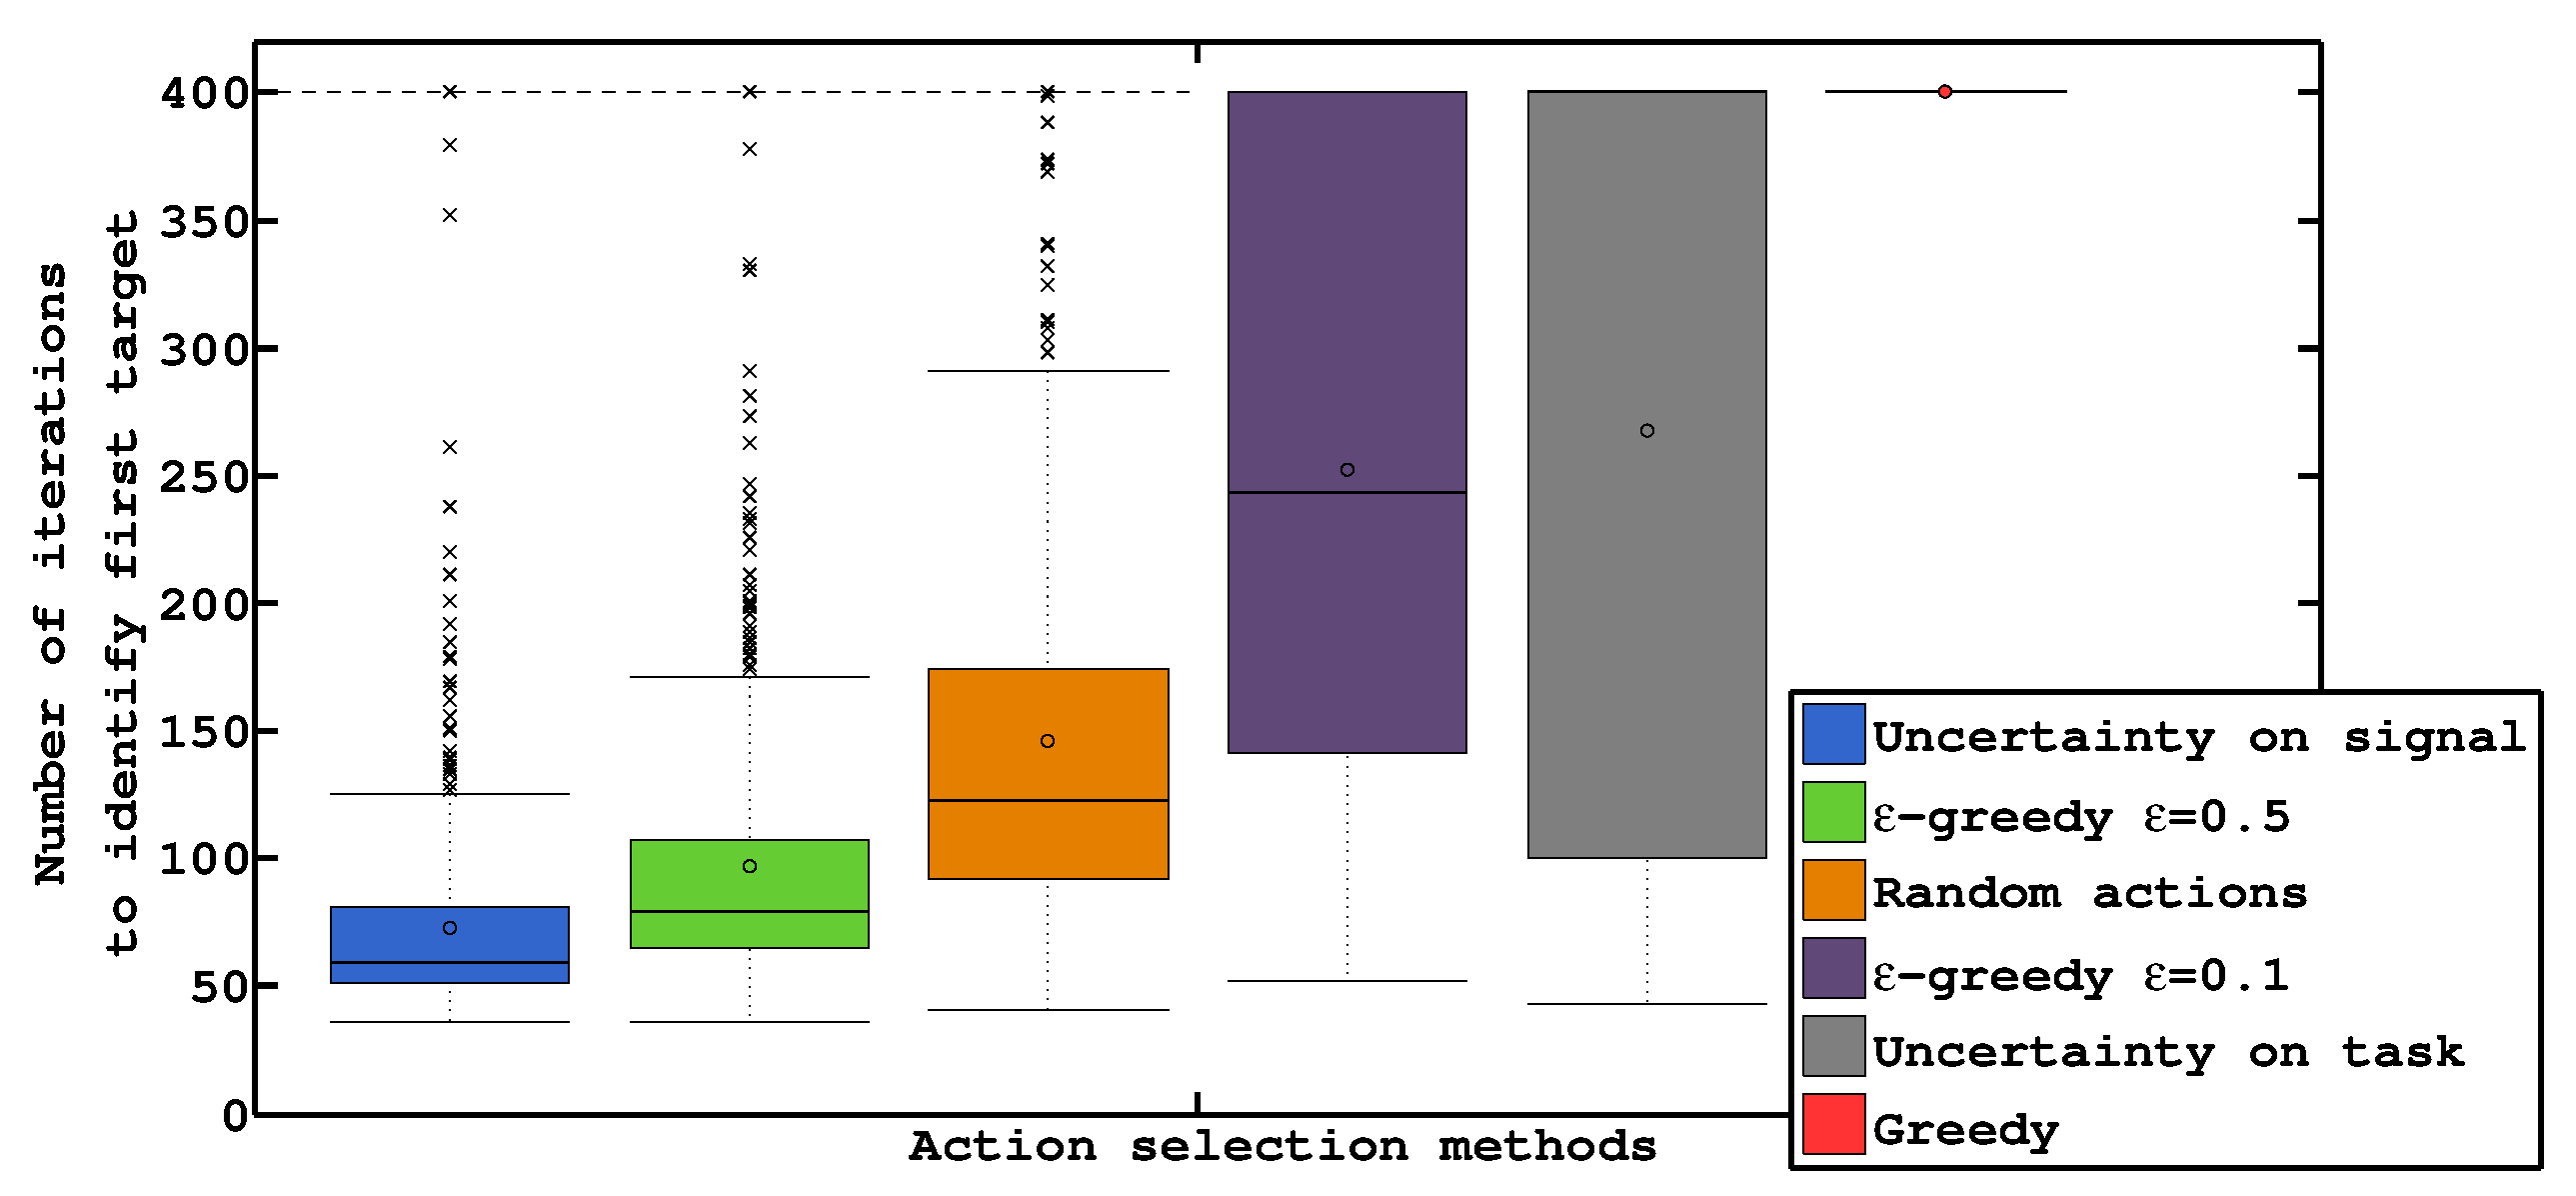
\includegraphics[width=\columnwidth]{\imgpath/battacharyya/plot_planning_first.eps}
    \caption{Comparison of different exploration methods. Our proposed method, based on the uncertainty on the expected signal, allows to lead the system to regions that improve disambiguation among hypotheses in a faster way. For the greedy method, all values were 400 which indicates it never allowed to identify any task.}
    \label{fig:overlapcompplan}
\end{figure}

Figure~\ref{fig:overlapcompplan} shows the results averaged across subjects, runs and datasets. Values of 400 means the confidence threshold was not reached after 400 iterations. Our proposed method, based on the uncertainty on the expected signal, allows to lead the system to regions that improve disambiguation among hypotheses in a faster way. Trying to follow the most probable task does not allow the system to explore sufficiently (Greedy), and at least some random exploration is necessary to allow a correct identification of the task ($\epsilon$-greedy). Assessing uncertainty only on the task performs poorly as it does not take into account the signal interpretation ambiguity inherent to our problem. The large variability in the results is mainly due to the large variations in classification accuracy across subjects and datasets. Given these results, the remainder of this section will only consider our proposed planning method.

\paragraph{Using the Bhattacharyya coefficient in the long run}

After identifying the first task, and following our approach, we continued running the system and measured how many tasks were identified after 400 steps. Figure~\ref{fig:overlapbhatta} demonstrates the advantage of switching to a classification based method after identification of a first target instead of keeping the estimation given by the Bhattacharyya coefficient. On the one hand, Bhattacharyya coefficient works very well for small amounts of data because it directly compares model parameters. On the other hand, after identifying many task, all models share most of their signal-label pairs and it requires much more data to modify the models and detect overlaps. Therefore using a classifier allows for a faster identification since the classifier makes a much harder decision for each new EEG signal. This discussion is in line with the observation on the use of the power information made in chapter~\ref{chapter:bci:priorpower}.

\begin{figure}[!ht]
    \centering
        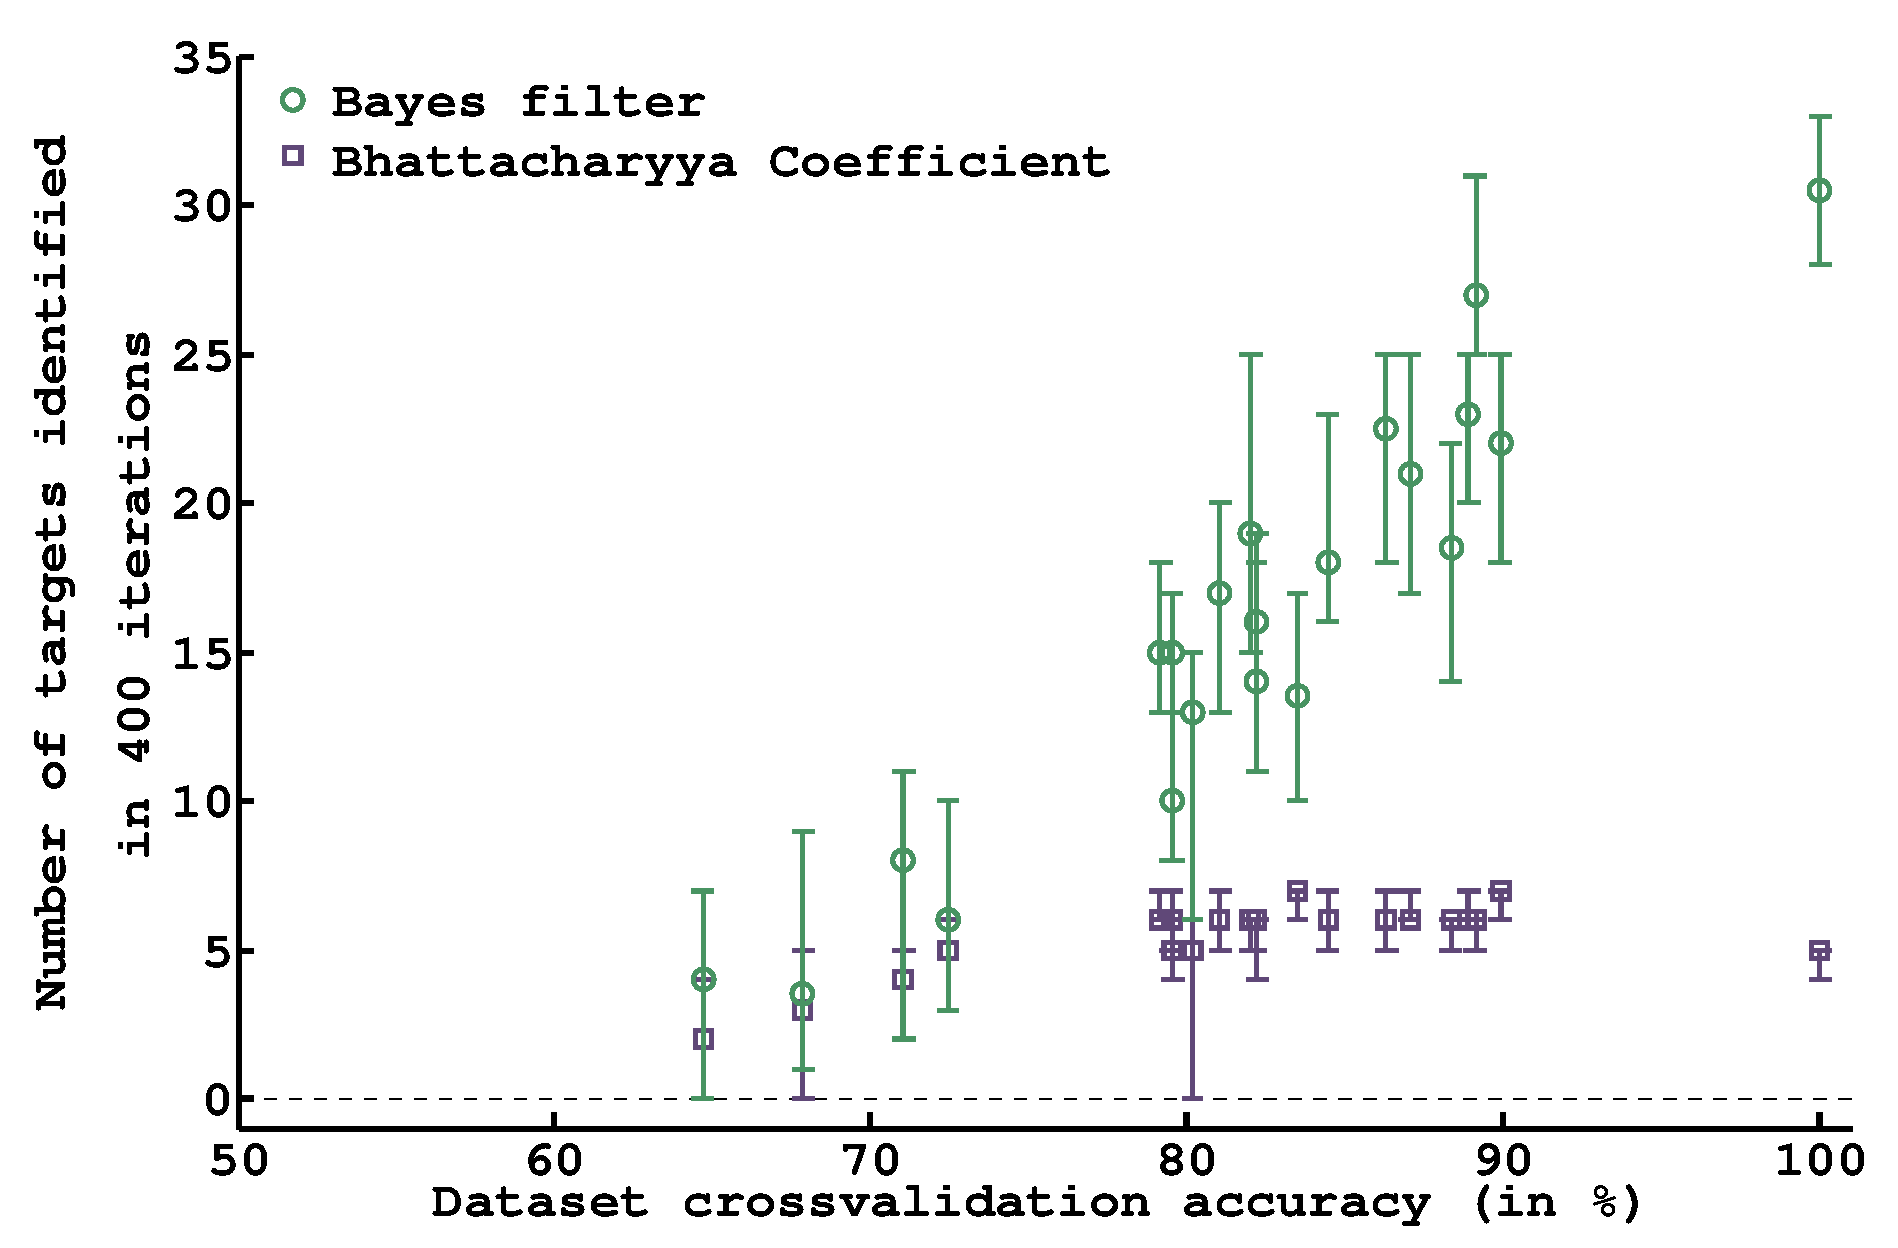
\includegraphics[width=\plotsize\columnwidth]{\imgpath/battacharyya/plot_bhattha_vs_bayes}
        \caption{Number of targets correctly identified in 400 iterations (the markers show the median values and the error bars the 2.5th and 97.5th percentiles). Comparison between switching to a Bayes filter method after identification of a first target instead of keeping the estimation given by the Bhattacharyya coefficient. The classification based method allows for a faster identification.}
        \label{fig:overlapbhatta}
\end{figure} 

Given these results, in the remaining of this section we only consider switching to a classification based method once the first task has been identified.

\paragraph{After 400 steps}

Figure~\ref{fig:overlapavg_sum_400} shows the number of tasks correctly and incorrectly identified in 400 iterations. For datasets of good qualities, we are able to identify more than 20 tasks in 400 iterations without the need for a calibration procedure (recap that previous works needed between 300 and 600 examples for the calibration phase \cite{chavarriaga2010learning,iturrate2010single}). The number of correctly identified tasks is strongly correlated to the quality of the dataset.

\begin{figure}[!ht]
    \centering
    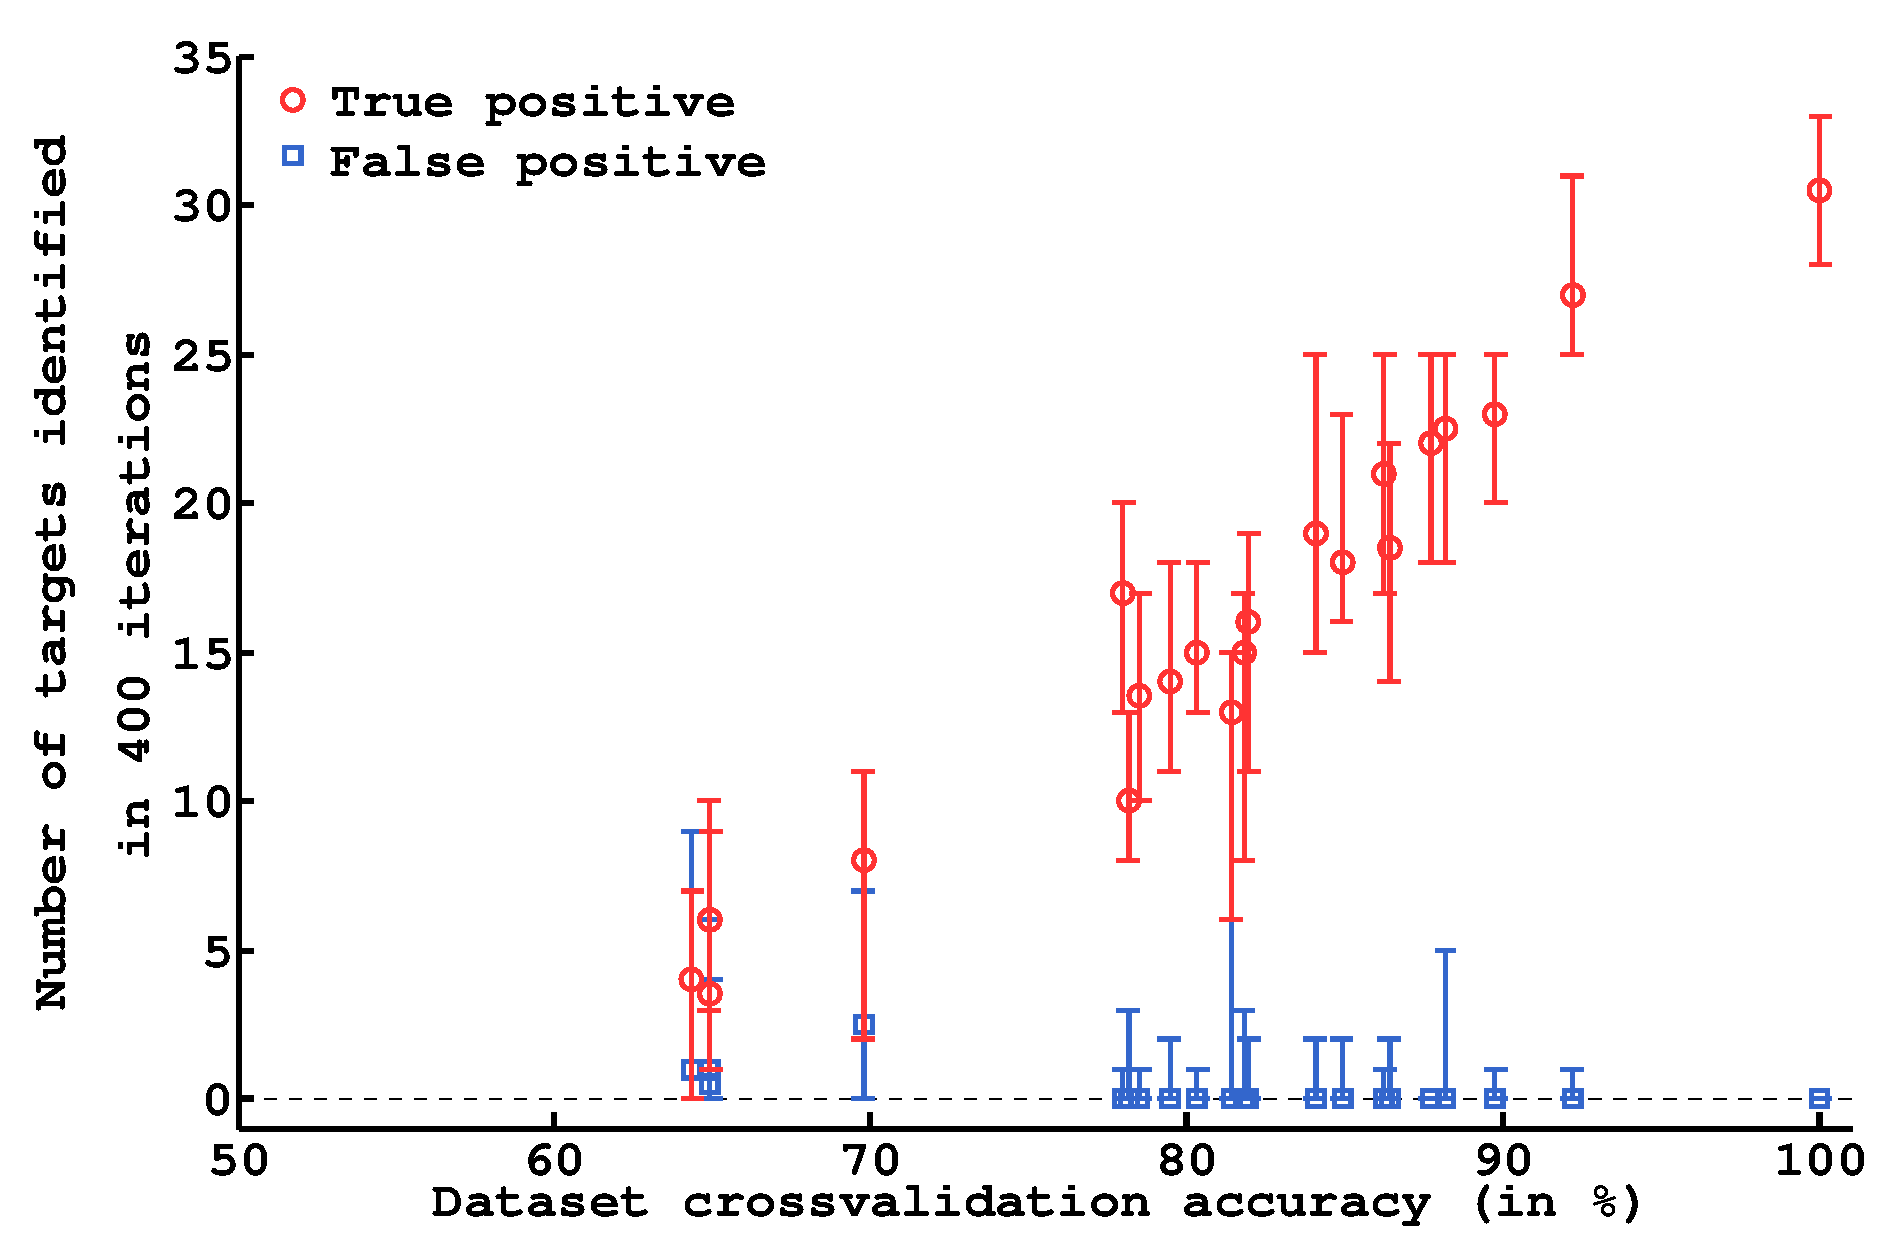
\includegraphics[width=\plotsize\columnwidth]{\imgpath/battacharyya/plot_first400_reach} 
    \caption{Number of targets correctly and incorrectly identified in 400 iterations (the markers show the median values and the error bars the 2.5th and 97.5th percentiles). For datasets of good qualities, we are able to identify more than 20 tasks in 400 iterations without the need for a calibration procedure.}
    \label{fig:overlapavg_sum_400}
\end{figure} 

The quality of our unsupervised method can be measured according to the percentage of labels correctly assigned (according to the ground truth label), see Figure~\ref{fig:overlappercentageLabels}. In general, having dataset with classification accuracies higher than 75$\%$ guaranteed that more than 90$\%$ of the labels were correctly assigned. This result shows that our algorithm can also be used to collect training data for calibrating any other state-of-the-art error-related potentials classifier, but has the important advantage of controlling the device at the same time.

\begin{figure}[!ht]
    \centering
        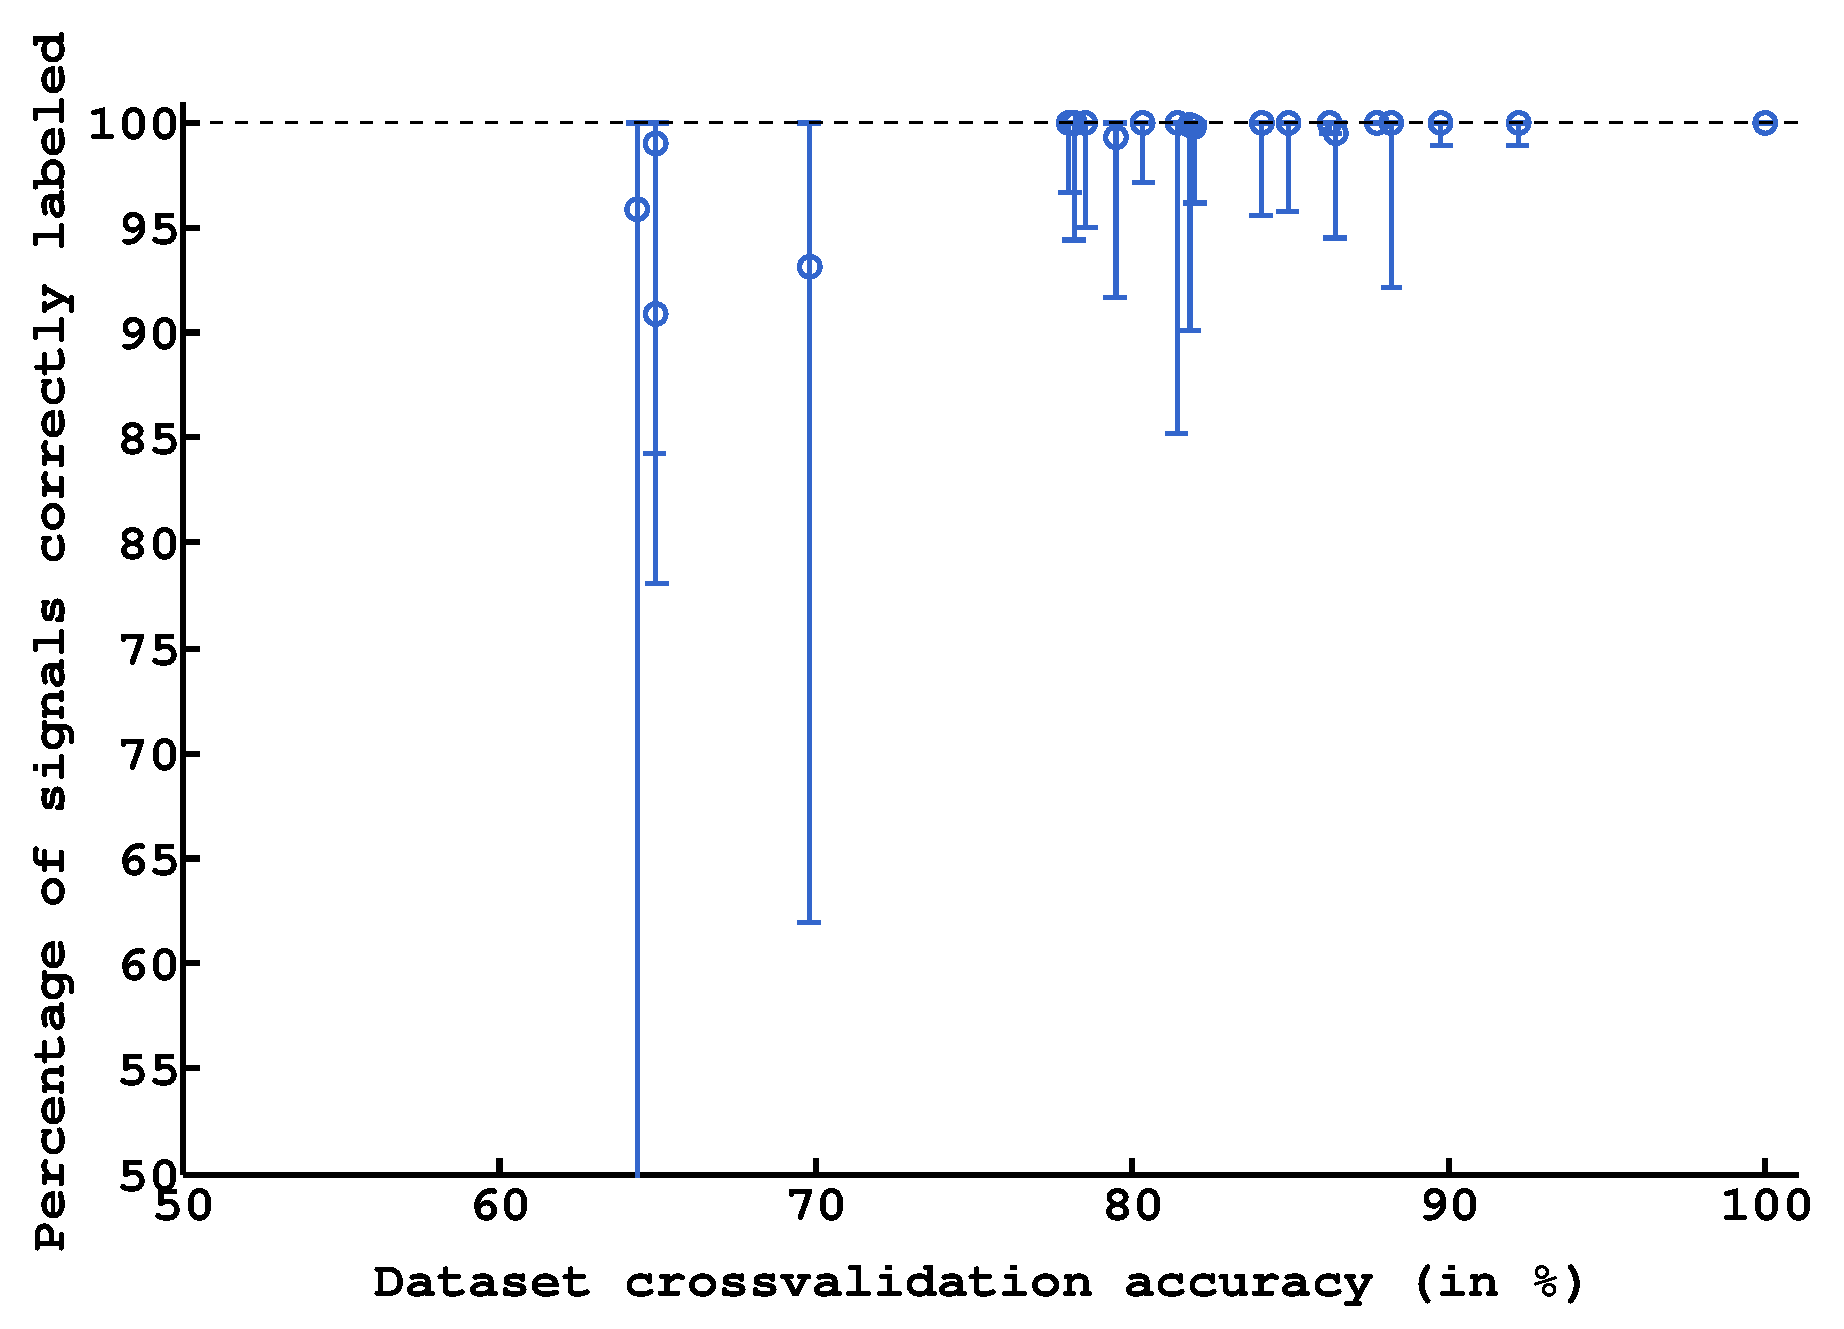
\includegraphics[width=\plotsize\columnwidth]{\imgpath/battacharyya/plot_percent_label}
        \caption{Percentage of labels correctly assigned according to the ground truth label (the markers show the median values and the error bars the 2.5th and 97.5th percentiles). In general, having dataset with classification accuracies higher than 75$\%$ guaranteed that more than 90$\%$ of the labels were correctly assigned.}
        \label{fig:overlappercentageLabels}
\end{figure}

\subsection{Online control}

The experiments were conducted with four subjects (aged between 25 and 28). Each subject was asked to mentally assess the agent's actions with respect to a given target. The system was not calibrated to decode the user EEG signals beforehand. Each subject performed 5 runs, for each run a new target was randomly selected and provided to the user. There was an action every three seconds. Each run lasted 200 actions, and the time between runs was around one minute.

The algorithm was able to identify the correct target for all runs of all the subjects, see Figure~\ref{fig:overlaponlineresults}. There are strong variations among subjects but we note that our system identified each task in less iterations than a normal calibration phase requires (between 300 and 600 examples depending on the user performance \cite{chavarriaga2010learning,iturrate2010single}).

\begin{figure}[!ht]
    \centering
    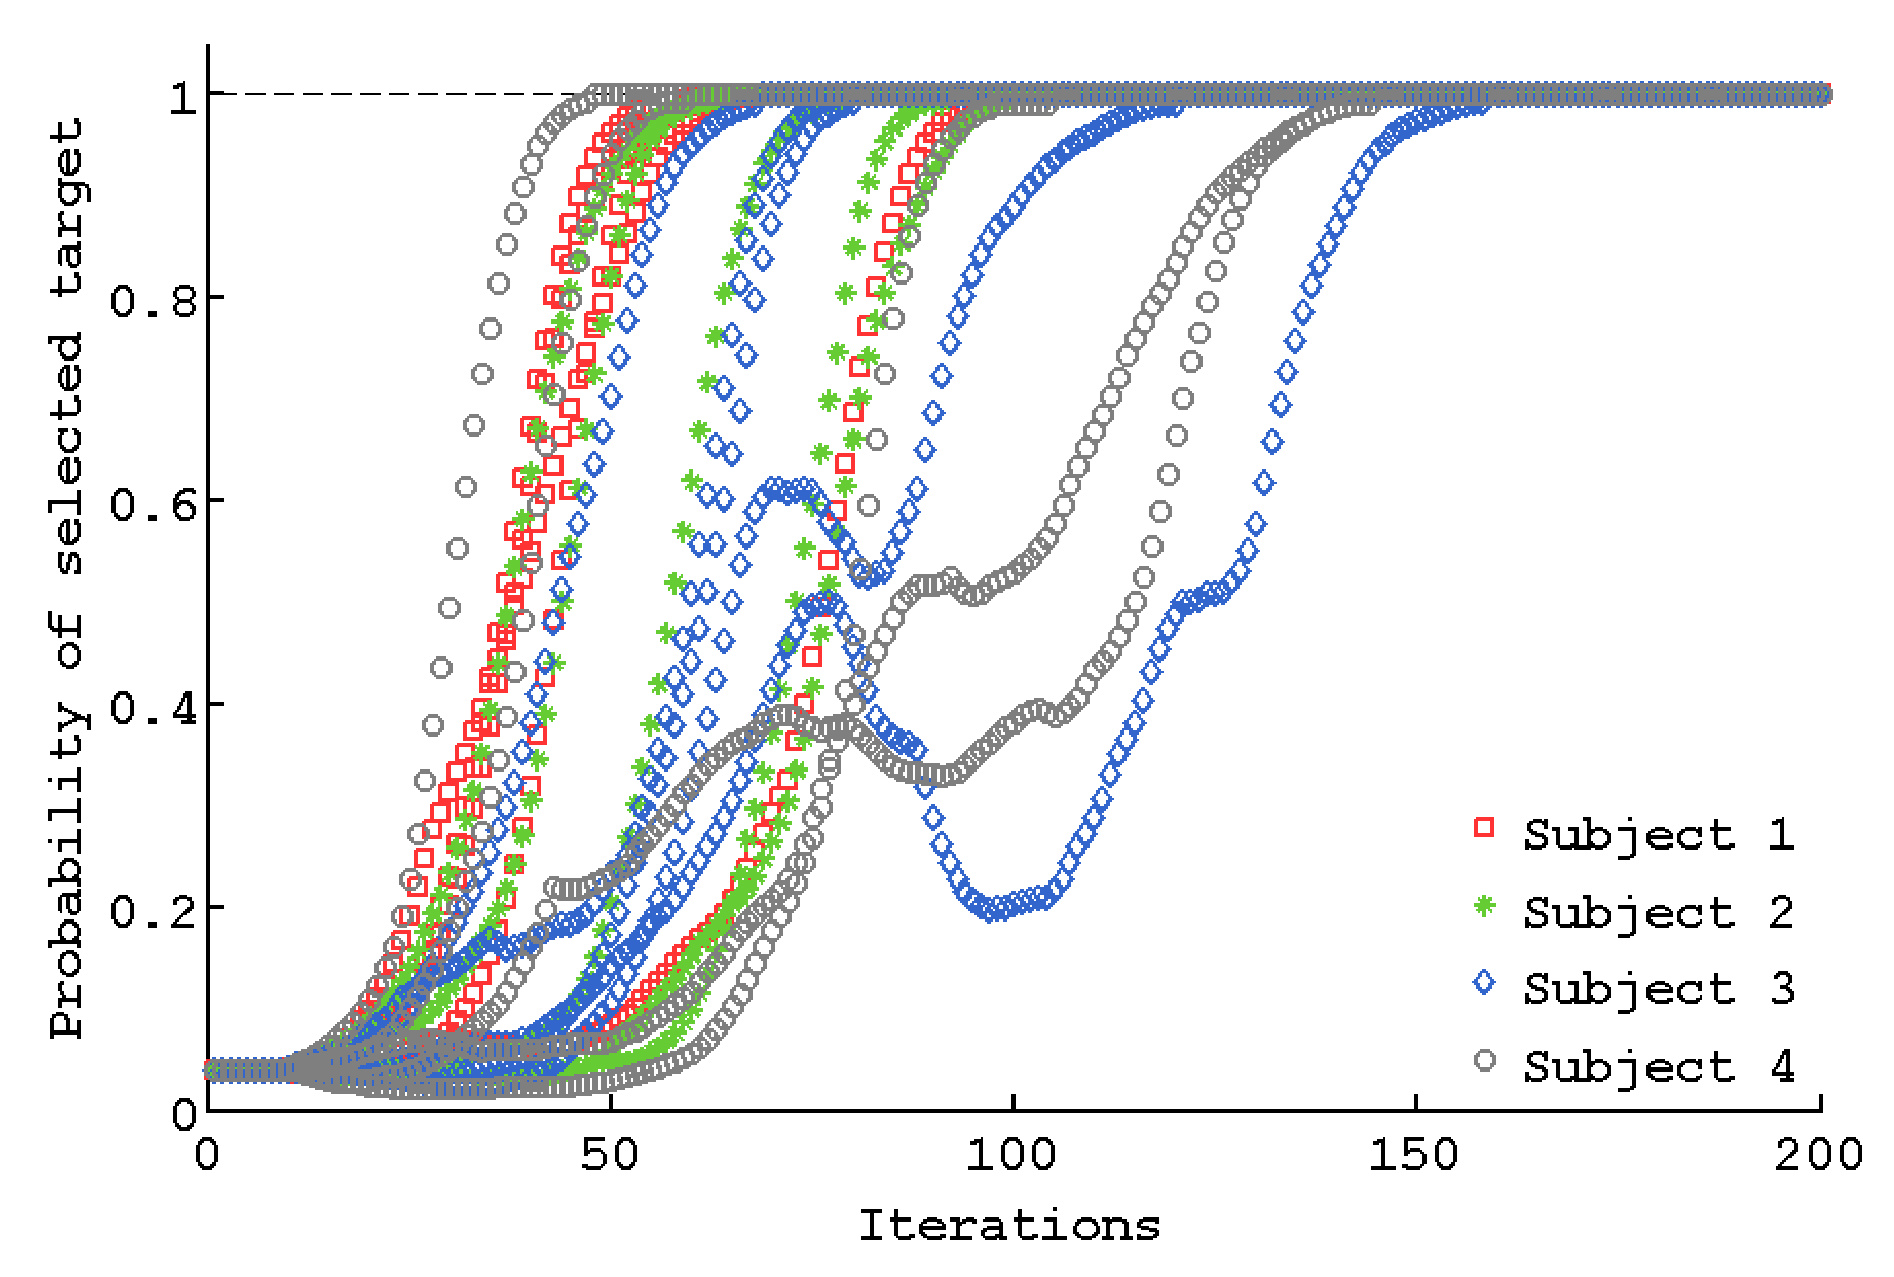
\includegraphics[width=\plotsize\columnwidth]{\imgpath/battacharyya/plot_realevolution}    
    \caption{Results from the online experiments: Evolution of the probability of the correct task for each subject and run. The algorithm was able to identify the correct target for each subjects and runs in less than 200 iterations.}
    \label{fig:overlaponlineresults} 
\end{figure}

Table~\ref{tab:overlaponline} shows for each subject and run the number of iterations needed to reach the confidence threshold for the subject selected target.

On average, the number of iterations needed to identify the target was of 85 $\pm$ 32.

\begin{table}[!ht]
\centering
\rowcolors{2}{gray!25}{white}
\begin{footnotesize}
\begin{tabular}{r|rrrrr|r}
    %\toprule
    & \textbf{Run1} & \textbf{Run2} & \textbf{Run3} & \textbf{Run4} & \textbf{Run5} & \textbf{mean$\pm$std} \\\hline
    %\midrule
    \textbf{S1} & 95 & 62 & 56 & 60 & 64 & 67 $\pm$ 16 \\
    \textbf{S2} & 89 & 77 & 98 & 60 & 62  & 77 $\pm$ 17 \\
    \textbf{S3} & 68 & 80 & 118 & 76 & 157 & 100 $\pm$ 37 \\
    \textbf{S4} & 98 & 142 & 57 & 142 & 47 & 97 $\pm$ 45 \\
\end{tabular}
\end{footnotesize}
  \caption{Results from the online experiments: Number of iterations needed to identify the correct target for each subject and run. On average, the number of iterations needed to identify the target was of 85 $\pm$ 32.}
  \label{tab:overlaponline}
\end{table}

\subsection{Discussion}

We introduced a new method to exploit the facts that, when associated hypothetic labels to all task hypothesis, only the correct task assign the correct labels to the correct hypothesis. This method compares directly the overlap between the distribution modeling the generation of such signals. As for wrong hypothesis, the labels tend to be mixed with respect to the underlying structure of the data, the overlap between distribution is a good and stable measure. 

However, we have seen that once all hypothesis share the same signal-label pairs, this method requires to collect more and more data to detect a change in the overlap of the wrong hypothesis. As a consequence the system should make use of two different sets of equations, one specific to the first target and one for the forthcoming targets.

This latter aspect shows the important advantage of the method we presented in this thesis, which only make use of one equation from the first to the last iteration. This equation captures both phase of the interaction, where during a first phase the classifier qualities are playing a major role, and in a second phase the classifier predictions are taking the lead by taking more hard decisions.